\section{Kostenrechnung}
Übersicht: s. FS4/13
\subsection{Kostenartenrechnung}
\textbf{Frage}: Welche Kosten sind in welcher Höhe in einer Periode angefallen? 
$\rightarrow$ Aufteilung auf Kostenarten

\textbf{Kostenarten}: Kategorie von Kosten, die nach bestimmten Kriterien aufgegliedert werden können

\textbf{Kostenartenhauptgruppen}: Personal- und Sozialkosten, Sach- und Materialkosten
Dienstleistungskosten, Kosten für Lizenzen, Kapitalkosten, öffentliche Abgaben und Steuern, Versicherungskosten und kalkulatorische Wagniskosten

\textbf{Variable Kosten}: Kosten, die mit der Ausprägung (Stückzahl) eines Kostentreibers variieren

\textbf{Fixe Kosten}: Kosten, die unabhängig vom Kostentreiber immer in konstanter Höhe anfallen

\textbf{Kostentreiber}: Variable, die am besten erklärt, wie die gesamten Kosten eines Kostenobjektes zustande kommen, z.B. Produktionsvolumen, Lieferungen, $\ldots$

\textbf{Break-even-Analyse}:
\begin{center}
	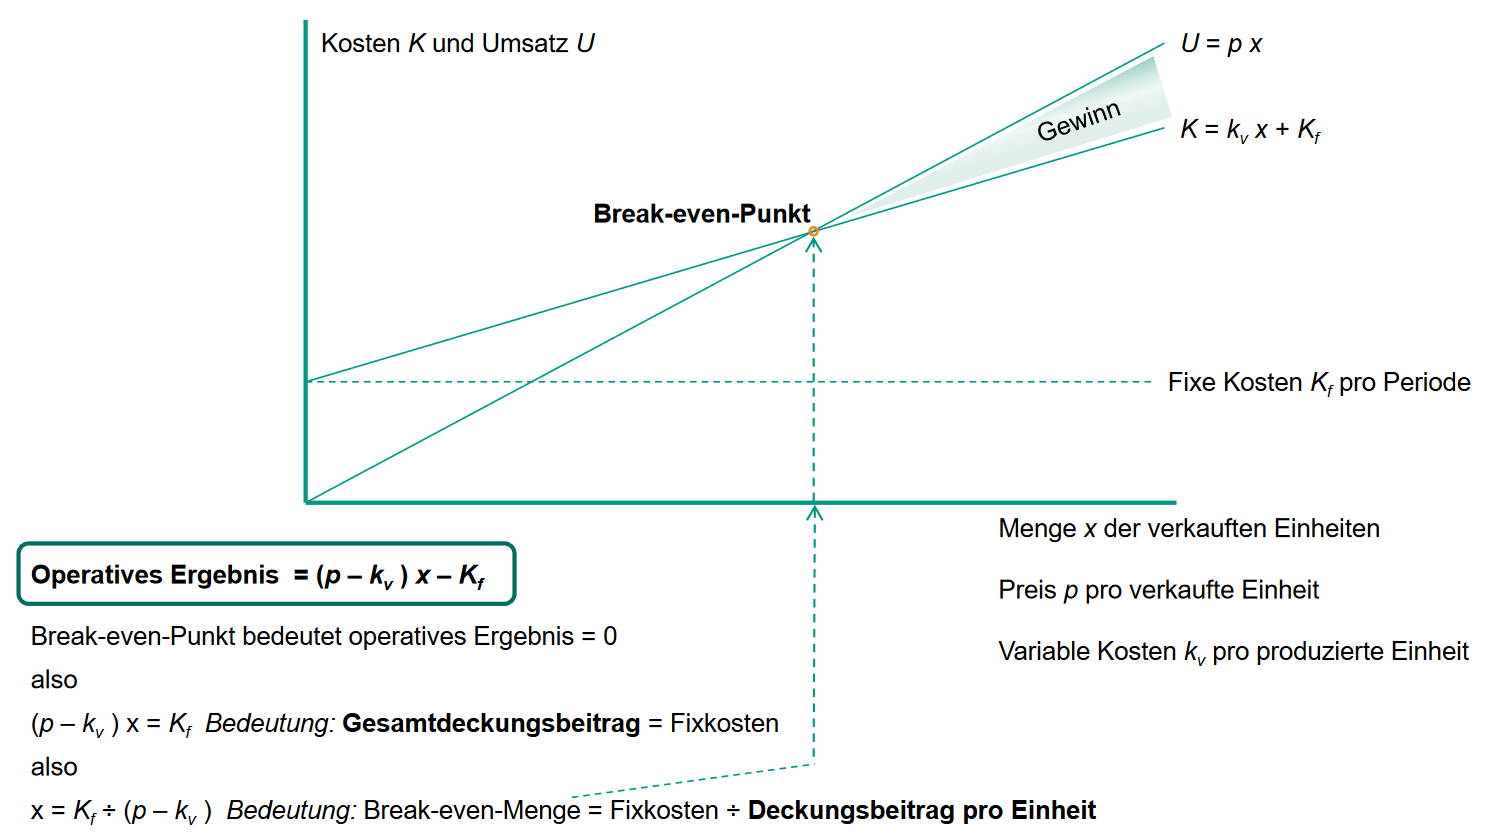
\includegraphics[width=\textwidth]{images/be-analyse.png}
\end{center}
$\text{Gewinn}=p\cdot x-k_V\cdot x-K_f$ \qquad\qquad\qquad\qquad\qquad\qquad\textit{Bsp. s. FS4/21}
\bigskip

\textbf{Einzelkosten}: Können einem Kostenobjekt eindeutig und vollständig zugeordnet werden

\textbf{Gemeinkosten}: Werden durch mehrere Kostenobjekte gemeinsam erzeugt $\rightarrow$ müssen indirekt über sinnvolle Kostenverteilungsschlüssel aufgeteilt werden

\textbf{Kostenobjekt}: Alles, wonach die Frage nach Kosten Sinn ergibt, z.B. Auftrag, Dienstleistung, Kunde, Standort.\\
$\rightarrow$ Einteilung in variable/fixe/Einzel-/Gemeinkosten nicht immer eindeutig!

\textbf{Ist-Kosten}: Bisher tatsächlich angefallene Kosten

\textbf{Plan-Kosten}: Zukünftig zu erwartende Kosten

\textbf{Normalkosten}: Durchschnittliche Ist-Kosten mehrerer vergangener Perioden
